\chapter{Feature selection}

Data collection is simply a process of fetching the data from the data source. However, feature selection is a process of selecting fields from which the target field will be predicted. Suppliers provide stock details along with associated product taxonomy. Importing well-defined taxonomy requires to train the classification model with already existing correct pair of features and label. The already existing pair of features and the correct label for each input is the training data set or training corpora. The classifier built on such a training corpora is termed as supervised classification \parencite{BirdKleinLoper09}.

\begin{figure}[H]
      \centering    
      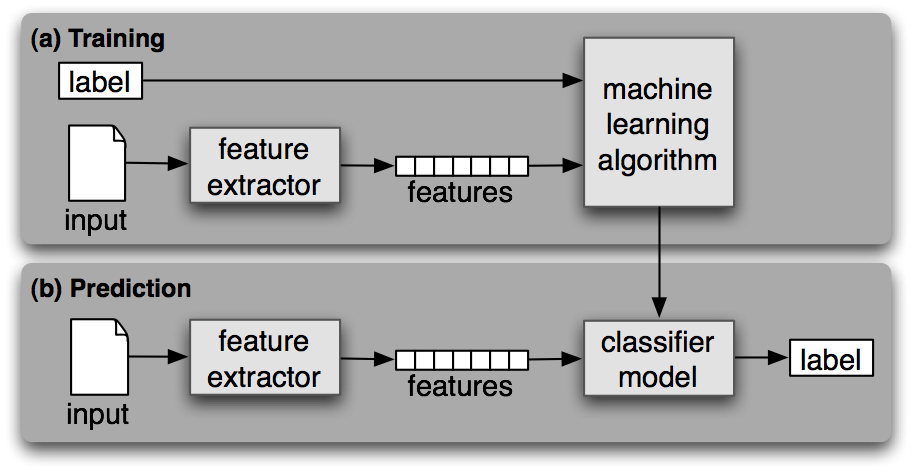
\includegraphics[scale=0.9]{supervised-classification.png}
      \caption{Supervised classification \parencite{BirdKleinLoper09}}
      \label{fig:supervised-classification}
  \end{figure}

  As illustrated in figure \ref{fig:supervised-classification}, during training, a pair of feature set and label are fed in to the machine learning algorithm to generate a classifier model. During prediction, same feature set are fed into the model to predict the label. Refer to chapter \ref{ch:feature-extraction} for details on feature extraction.

In this project, author choose to create a classification model with only one feature that is the name of the product. However, author identifies the potential features to classify the target of n levels of category. These features have been identified based on the understanding of domain of the product. For products with many details will have many more features to be taken into consideration. In such case, selection based on common understanding of the nature of the product may not be sufficient. Hence, Scikit learn  \parencite{sklearn_api} provides methods to define feature appropriately. 


\section {Feature selection methods} \label{sec:feature-selection}

A feature represents a dataset fine-tuned to serve as a training data for machine learning model. Choosing obvious set of features could get a decent performance on classification task. However, carefully constructed relevant set of features could impact the learning ability and have a significant gain in performance. The feature selection API from Scikit learn \parencite{sklearn_api} also refers to it as dimensionality reduction. 

\parencite{BirdKleinLoper09}  describes some approaches for feature selection as following:

\begin{itemize}
      \item Kitchen sink 
      

      All the features are initially included later each are checked to determine whether they are actually helpful.

      \item Error analysis
      
      The data corpus is split into development-set and test-set. Development-set is subdivided into training set and dev-test set. Training set is used to train the model, dev-test set is employed for error analysis.  The individual error cases are examined for wrongly predicted labels.
      
      
      \begin{figure}[H]
            \centering    
            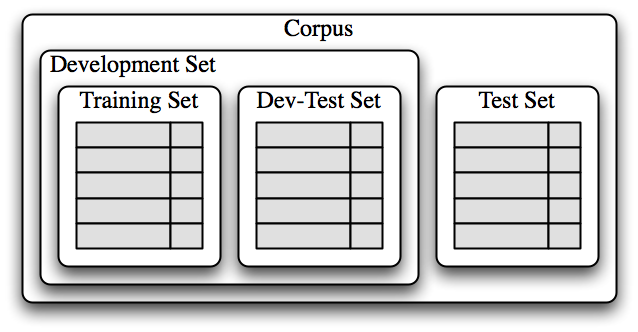
\includegraphics[scale=0.5]{corpus-org.png}
            \caption{Corpus organization for supervised classification \parencite{BirdKleinLoper09}}
            \label{fig:corpus-supervised-classification}
        \end{figure}

\end{itemize}

 Methods for feature selection with Scikit Learn API are:-
\begin{itemize}
      \item Removing features with low variance
      \item Univariate feature selection
      \item Recursive feature elimination

\end{itemize}

\section{Obvious feature selection}

In this paper, the datasets used are of an ecommerce business specializing in automotive industry domain. Secondary dataset used is from the TecDoc catalogue by TecAlliance \footnote{https://www.tecalliance.net/}. 

Table \ref{table:feature_decription} lists the obvious features for an ecommerce domain. In this paper, five levels of categories are taken into consideration. The number of category levels differ for each product. Consider an example of category tree with three levels. 

\begin{quote} 
\centering 
sparepart/cooling-system/thermostat
\end{quote}
In this example, the lowest level of category is ``thermostat'' as level 4 and level 5 does not exist and will be represented by black or NaN. These blank or NaN value records can go through data imputation as discussed in chapter \ref{ch:data-imputation}.



\begin{table}[h]
      \centering
      \caption{Feature description}
      \label{table:feature_decription}
      \begin{tabular}{ lll }
            \toprule
            
            \textbf{No}& \textbf{Feature} & \textbf{Description}\\
            \midrule
            1&Product name & normalized form of name\\
            2&Category tree & multi level categories\\
            3&Description & Description with html tags\\         
            4&Short description  & product info displayed\\
            5&Supplier  &  supplier of the product\\
            6&Manufacturer  &  manufacturer of the product\\           
            7&Price  &  Price of the product\\
            8&Dimension  & Height, weight of the product\\
            9&(n-1) number of  category levels   &  n is the total category level, one of which will be the target\\
           
            \bottomrule
            \end{tabular}


\end{table}

\section {Fetch existing product taxonomy (Corpus) using Elasticsearch}
Elastic search \footnote{https://www.elastic.co/} is a fast and scalable search and analytics engine. It can build a powerful AI and machine learning enabled search experience. In this paper, author fetches labeled dataset of products to serve as the training data for the machine learning model.
For this project, python client elasticsearch 6.8.2 is installed as the client needs to be compatible with Elastic search version being used. The official Python client provides mapping with Elasticsearch REST APIs.

\begin{lstlisting}[language=Python]
resp=self.es.search("english-name-category",{"_source":["id","name","category"],
'from':_from,
'size' :_size ,
"query": {"match_all": {}}})
\end{lstlisting}

The above code fetches indexed product name and its lowest hierarchy level category.  
\begin{table}[h]
      \caption{Index: english-name-category statistics}
      \centering
      \label{table:enc}
\begin{tabular}{ll}
      \toprule 

      Samples total&22160 \\
      Dimensionality&2 \\
      Features&name \\
      Label&category \\
      
      \bottomrule
\end{tabular}
\end{table}

Table \ref{table:enc} highlights the total number of products and category and name of fields considered as feature and label. 


\section{Summary}

In this chapter, search analytic engine named Elastic search is introduced. The author as a prototype of classification model choose to include only two-dimensionality. One is the feature (product name) and other is the label to be predicted (category.)

Table \ref{table:feature_decription} list the features for determining the product taxonomy. These features are listed based on general knowledge and understanding. However, productive method for refining the feature such as error analysis can be utilized for feature selection. Scikit learn API \parencite{sklearn_api} also provides some functions for feature selection.